\documentclass[a4paper,english,11pt,twoside,openright]{book}
\usepackage{babel}
\usepackage[T1]{fontenc}
\usepackage[latin1]{inputenc}

%\usepackage{babel}
%\usepackage[lining]{minion}
\usepackage[oldstyle]{minion}
%\usepackage[T1]{fontenc}
%\usepackage[latin1]{inputenc}
%\usepackage{palatino}
%\usepackage{mathpazo}
\usepackage{amsmath,amsfonts,amssymb}
\usepackage{titlesec}
\usepackage{achicago}
\usepackage{calc}
\usepackage[mathcal]{euscript}
\usepackage[leftno,noindent,norules]{lgrind}
\usepackage{layout}
\usepackage{subfigure}
\usepackage{synttree}
\usepackage{varioref}
\usepackage{color}
\usepackage{booktabs}

\usepackage{graphics}
\usepackage[dvips]{graphicx}
\usepackage{epsfig}

\usepackage{longtable}

\bibliographystyle{achicago}

\usepackage{index}

\usepackage{concept}
%\def\persondef#1[#2]#3{}
%% $Id$
%
\chapter*{Abbreviations}
\addcontentsline{toc}{chapter}{\numberline{}List of Abbreviations}

\begin{longtable}[l]{@{}ll@{}}
  %\caption{Results of first large simulation.}\\
  %\toprule
  %Acronym & Meaning \\
  %\midrule
  \endhead
  %\bottomrule
  \endfoot
  \input{alist.txt}
\end{longtable}

%\begin{multicols}{2}
%\begin{tabular}{@{}lp{.30\textwidth}@{}}
%\input{alist.txt}
%\end{tabular}
%\end{multicols}


% Local Variables:
% mode: latex
% eval: (set-default 'ispell-local-dictionary "english")
% mode: flyspell
% comment-column:0
% comment-start: "%"
% comment-end: ""
% TeX-master: "main"
% End:

%\input{persons}
%\newcommand{\coa}[1]{\emph{#1}}
%\newcommand{\cop}[1]{\emph{#1}}
\renewcommand{\cofont}[1]{\emph{#1}}
\renewcommand{\coafont}[1]{\emph{#1}}
\renewcommand{\copfont}[1]{\textsl{#1}}

% Indexing commands.
\def\DefaultIndex{Index\xspace}
\newindex{default}{ddx}{dnd}{\DefaultIndex}

\def\SrcIndex{Function Index\xspace}
\newindex{src}{sdx}{snd}{\SrcIndex}

% Definition of acronyms used throughout the text.
\acrodef{CPU}{central processing unit}
\acrodef{I/O}{input/output}
\acrodef{TAD}{TUC Alert Daemon}
\acrodef{TTPD}{TUC Transfer Protocol Daemon}
\acrodef{TUC}{The Understanding Computer}
\acrodef{SMS}{Short Message Service}

\title{TUC Transfer Protocol Daemon \\ \textit{\&} \\ TUC Alert
  Daemon: \\[2em] System Documentation}

\author{Martin Thorsen Ranang}

\newcommand{\code}[1]{\texttt{#1}}

\begin{document}

\frontmatter
\maketitle

\tableofcontents
\listoffigures
\listoftables

%\input{preface}
%\input{acknowledgments}

% $Id$
%
\chapter*{Abbreviations}
\addcontentsline{toc}{chapter}{\numberline{}List of Abbreviations}

\begin{longtable}[l]{@{}ll@{}}
  %\caption{Results of first large simulation.}\\
  %\toprule
  %Acronym & Meaning \\
  %\midrule
  \endhead
  %\bottomrule
  \endfoot
  \input{alist.txt}
\end{longtable}

%\begin{multicols}{2}
%\begin{tabular}{@{}lp{.30\textwidth}@{}}
%\input{alist.txt}
%\end{tabular}
%\end{multicols}


% Local Variables:
% mode: latex
% eval: (set-default 'ispell-local-dictionary "english")
% mode: flyspell
% comment-column:0
% comment-start: "%"
% comment-end: ""
% TeX-master: "main"
% End:


%\input{abstract}


\chapter{Abstract}
\label{cha:abstract}

This document provides an overview of both the \coal{TTPD} and the
\coal{TAD} software.


\mainmatter

\chapter{Overview}
\label{cha:overview}

The main purpose of \coa{TTPD} is to work as a mediator for requests
between external programs and \coa{TUC}.  In addition, if used with
the \coa{TAD} it will also handle `alert'\footnote{That is, messages
  like ``Kan du varsle meg 15 minutter f�r bussen fra Nardo til
  Gl�shaugen g�r?''} requests when used in conjunction with the
\coa{SMS} interface.  Figure~\ref{fig:overview} shows an overview of
the system architecture.

Both programs were implemented in Python version 2.3.4.

\begin{figure}[htbp]
  \centering
  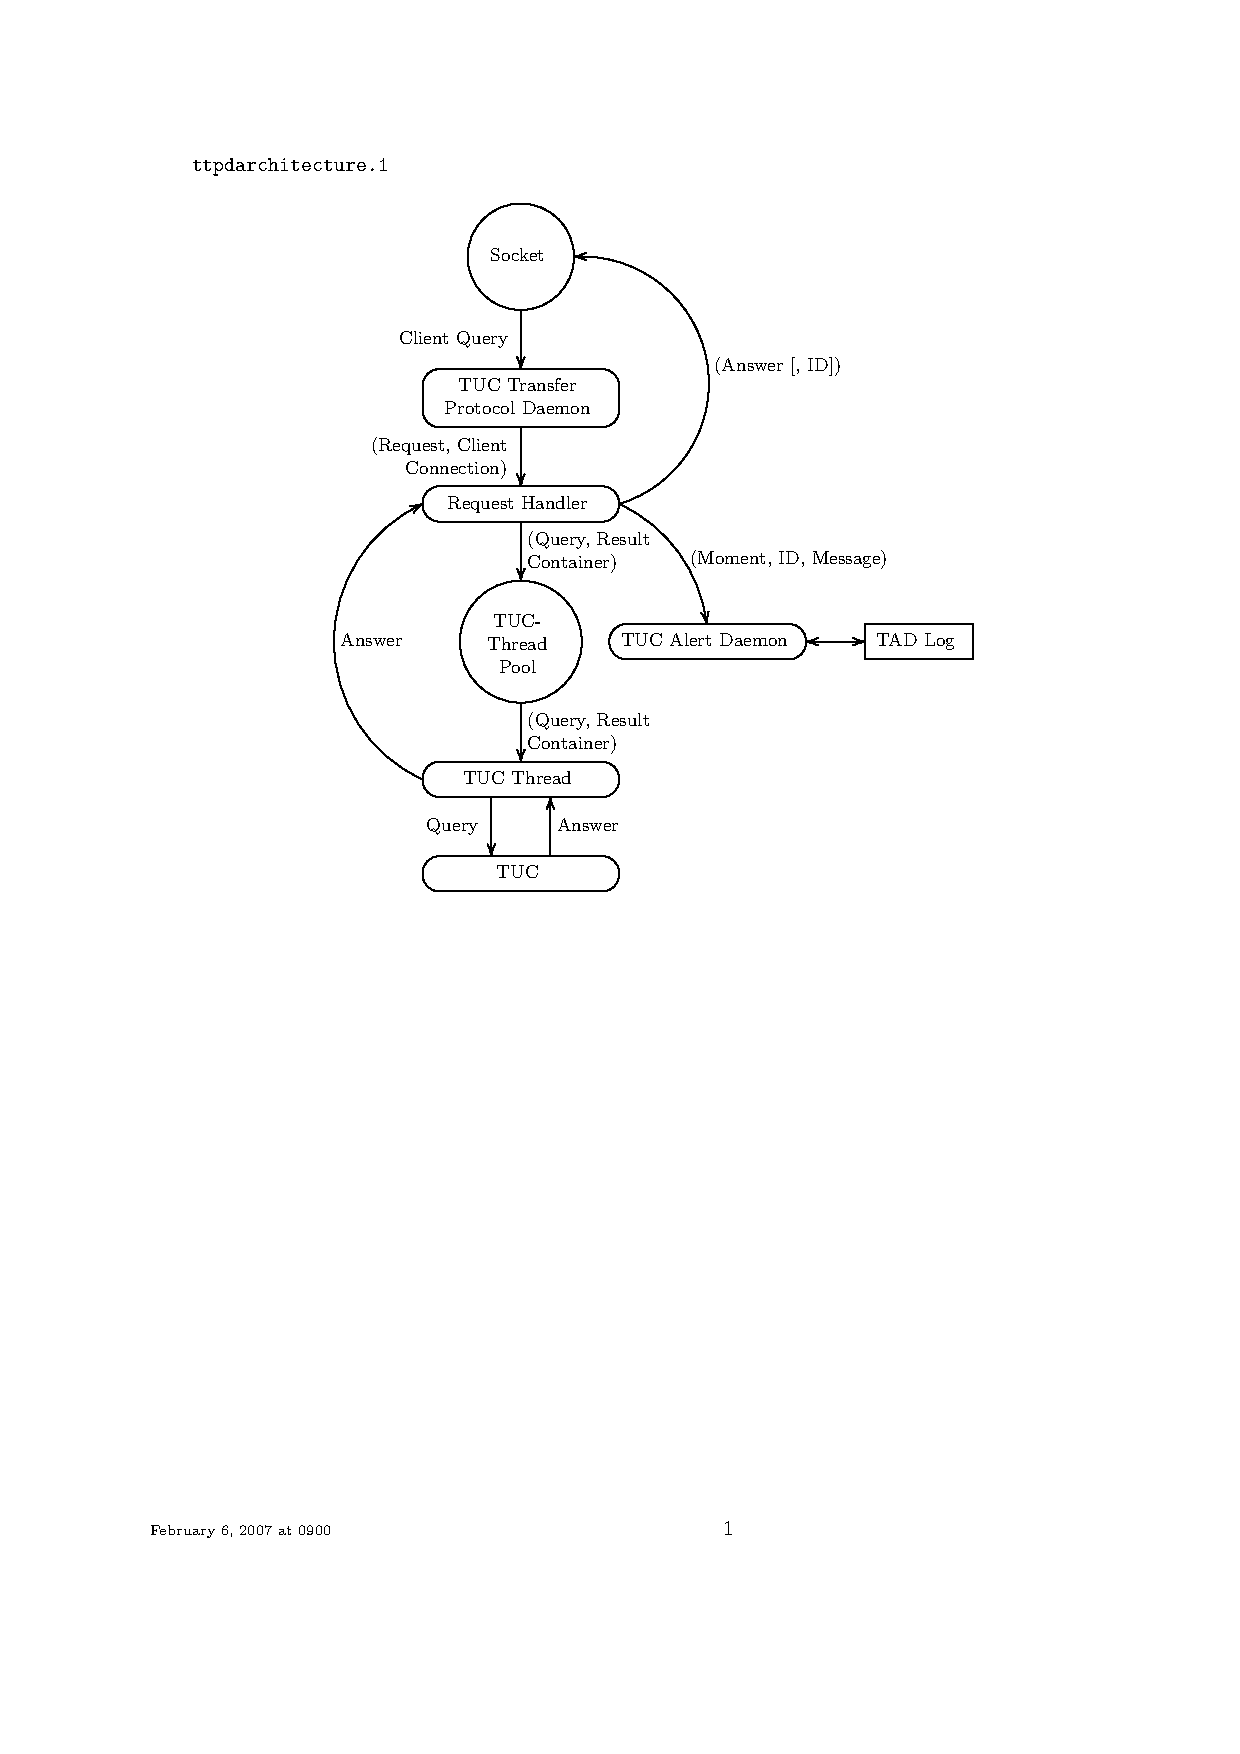
\includegraphics{ttpdarchitecture.1}  
  \caption{Overview of the \protect\coa{TTPD} and \protect\coa{TAD}
    system.}

  \label{fig:overview}
\end{figure}

\section{TUC Transfer Protocol Daemon}
\label{sec:tuc-transf-prot}

The \coa{TTPD} is implemented as a \co{threading} server, listening
for connections from \co{clients} on a user-specified network port (by
using a \co{socket}).  When a request is received, the server starts a
\co{handler thread} responsible for handling the request.  First, the
nature of the request is determined.  If it is an `alert cancellation'
request, the request is handled by the \co{handler thread} through
communication with \coa{TAD} and the \co{client} (see
Section~\ref{sec:tuc-alert-daemon} for more information about this
behavior).  However, if the request is not of that nature, it is
forwarded to \coa{TUC} for processing.  This is done by having the
server act as a \co{producer thread} that places incoming \co{tasks}
in a \co{thread pool} with $n \in \langle0, k]$ \co{consumer threads}.  Each
of the \co{consumer threads} controls \emph{one} external \coa{TUC}
process each.

The external \coa{TUC} processes are started by the server before it
starts accepting connections.  This is done because it would take too
long if an external \coa{TUC} process should be started in order to
handle each request.  In relation to the main server process, the
\coa{TUC} are \co{forked} processes.  The communication between each
\co{consumer} thread and its \coa{TUC} process is done through
\co{pipes} that function as the \coa{TUC} process' \code{stdin} and
\code{stdout} file streams.

When the result from \coa{TUC} has been received, the \co{consumer
  thread} stores it in a \co{thread-safe} container that only the
original \co{handler thread} and the \co{consumer thread} shares.
Hence, the response for handling the request is again returned to the
\co{handler thread}.  Now, the result is parsed, the appropriate
information is logged and an answer is given to the client.

\section{TUC Alert Daemon}
\label{sec:tuc-alert-daemon}

The \coa{TAD} is built-in as a part of \coa{TTPD}, but has its own
responsibilities.

The most central component of \coa{TAD} is a \co{scheduler}
responsible for the timing of sending out alert-messages at the
moments specified by users.

\coa{TAD} consists mainly of two threads that for the most of the time
run independently of the \coa{TTPD} process.  One thread constitutes
an \co{alert scheduler} while the other thread handles requests of
adding and removing alerts and is responsible for communicating with
the \co{database engine}.  The communication between a \co{TTPD
  request handler} and the \co{TAD request handler} is done through a
shared request pool (thread-safely protected by \coP{lock}).


\chapter{Design Criteria}
\label{cha:design-criteria}

The main goals of this work was to make the system more robust and to
implement an alert service.  In addition to this, where there have
been several possible solutions to a problem, the guiding principles
has been as follows: choose solutions that are \emph{easily
  maintainable} (use standard modules and programs if available, and
write easily readable code and documentation), \emph{highly scalable}
and that will \emph{probably not need to be changed} in the near
future.  In addition, the system has been designed in the spirit of
\con{Unix} philosophy; embracing modularity, the use of stream
redirection and process control as described
by~\citeN{ranang03:fragrance_of_unix}.  For a very concise
introduction to the theory and pragmatics of server/daemon design,
please see~\cite{327245,327308,327345}.


\section{Scalability and Robustness}
\label{sec:scalability}

The \co{scalability} of the system has been improved in several ways.
First of all, the design of \coa{TTPD} allows a computer to serve
multiple \coa{TUC} requests in parallel.  This is ensured through the
use of the pool of \co{TUC-threads} where each thread controls an
externally started \coa{TUC} process.  This means that if more
\coap{CPU} are added to the computer, each processes can run on its
own \coa{CPU}.  Even without multiple \coap{CPU}, the computer can
serve multiple requests in multiplexed parallel (but possibly with a
longer delay than when serving single requests, depending both on
\coa{CPU} and \coa{I/O} intensity).




%\input{introduction}
%\input{methods}
%\input{results}
%\input{discussion}

\appendix

\chapter{Source Code}
{
% A little hack to create a ``function index''.
\makeatletter%
\let\oldindex\index%
\newcommand{\mtrindex}[1]{%
\oldindex[src]{#1}%
}
\let\index\mtrindex%
\makeatother%
\input{src_doc/SocketServer-module}
\input{src_doc/TTP-module}
\input{src_doc/TTP.CoreMessage-module}
\input{src_doc/TTP.CorePayExMessage-module}
\input{src_doc/TTP.Definitions-module}
\input{src_doc/TTP.ESolutionsMessage-module}
\input{src_doc/TTP.EncapsulateTUC-module}
\input{src_doc/TTP.Handler-module}
\input{src_doc/TTP.LogHandler-module}
\input{src_doc/TTP.Message-module}
\input{src_doc/TTP.PayExMessage-module}
\input{src_doc/TTP.Server-module}
\input{src_doc/TTP.Statistics-module}
\input{src_doc/TTP.TUCThread-module}
\input{src_doc/TTP.ThreadPool-module}
\input{src_doc/TTP.daemon-module}
\input{src_doc/TTP.num_hash-module}
\input{src_doc/TTP.payex_prod-module}
\input{src_doc/TTP.payex_prod.PxSms_client-module}
\input{src_doc/TTP.payex_prod.PxSms_server-module}
\input{src_doc/TTP.payex_prod.PxSms_types-module}
\input{src_doc/TTP.payex_test-module}
\input{src_doc/TTP.payex_test.PxSms_client-module}
\input{src_doc/TTP.payex_test.PxSms_server-module}
\input{src_doc/TTP.payex_test.PxSms_types-module}
\input{src_doc/TTP.tad-module}
 % Include source-code listings.
\let\index\oldindex%
}

%\input{src_doc/SocketServer-module}
\input{src_doc/TTP-module}
\input{src_doc/TTP.CoreMessage-module}
\input{src_doc/TTP.CorePayExMessage-module}
\input{src_doc/TTP.Definitions-module}
\input{src_doc/TTP.ESolutionsMessage-module}
\input{src_doc/TTP.EncapsulateTUC-module}
\input{src_doc/TTP.Handler-module}
\input{src_doc/TTP.LogHandler-module}
\input{src_doc/TTP.Message-module}
\input{src_doc/TTP.PayExMessage-module}
\input{src_doc/TTP.Server-module}
\input{src_doc/TTP.Statistics-module}
\input{src_doc/TTP.TUCThread-module}
\input{src_doc/TTP.ThreadPool-module}
\input{src_doc/TTP.daemon-module}
\input{src_doc/TTP.num_hash-module}
\input{src_doc/TTP.payex_prod-module}
\input{src_doc/TTP.payex_prod.PxSms_client-module}
\input{src_doc/TTP.payex_prod.PxSms_server-module}
\input{src_doc/TTP.payex_prod.PxSms_types-module}
\input{src_doc/TTP.payex_test-module}
\input{src_doc/TTP.payex_test.PxSms_client-module}
\input{src_doc/TTP.payex_test.PxSms_server-module}
\input{src_doc/TTP.payex_test.PxSms_types-module}
\input{src_doc/TTP.tad-module}


%\input{ideas}
%\input{non_public}

%\nocite{*}

\bibliography{bibliography}


%% The function index.
\newpage{\thispagestyle{empty}\cleardoublepage}
\addcontentsline{toc}{chapter}{\numberline{}\SrcIndex}
\printindex[src]

%% The main index.
\newpage{\thispagestyle{empty}\cleardoublepage}
\addcontentsline{toc}{chapter}{\numberline{}\DefaultIndex}
\printindex[default]

\end{document}

%%% Local Variables: 
%%% mode: latex
%%% buffer-file-coding-system: latin-1-unix
%%% TeX-master: "ttpd_documentation"
%%% mode: flyspell
%%% End: 
